%%%%%%%%%%%%%%%%%%%%%%%%%%%%%%%%%%%%%%%%%%%%%%%%%%%%%%%%%%%%%%%%%%%%%%%%%%%%%%%%
%% 
\cleardoubleoddpage%  Make sure to start each chapter on a new odd page
\chapter{Anforderungen, Systemarchitektur und Datenmodell}
\section{Anforderungen}
Basierend auf bereits bestehenden Implementierungen sowie konkreten Anforderungen des Krankenhauses wurden die Systemanforderungen definiert. Das Projekt wird als Full-Stack-Webanwendung umgesetzt und ist über den Webbrowser zugänglich. Dabei kommen folgende Technologien zum Einsatz:
\begin{table}[h]
	\centering
	\caption{
		Technologien
	}\label{tab:nicetable}
	\begin{tabularx}{\linewidth}{l>{\raggedright\arraybackslash}X}
		\toprule
		\textbf{Subsystem}        & \textbf{Konkrete Technologie} \\
		\midrule
		\texttt{Frontend}     & Angular \\
		\texttt{Backend}      & FastAPI \\
		\texttt{Datenbank} & PostgreSQL / Supabase \\
		\texttt{ASP-Solver}      & Clingo \\
		\bottomrule
	\end{tabularx}
\end{table}

Das System soll die Erstellung eines Monatsplans von der Pflegeleitung für Mitarbeiter in einer Abteilung in einem Krankenhaus ermöglichen. Für jeden Mitarbeiter soll die Anzahl der Arbeitstage pro Monat erfasst werden können. Im Rahmen dieser Arbeit wird ausschließlich eine Tagesschicht betrachtet, unterschiedliche Schichtarten werden daher nicht berücksichtigt.

Zusätzlich müssen verschiedene Hard Constraints eingehalten werden. Ein Mitarbeiter darf an einem Tag nur einer Station zugeteilt werden. Außerdem darf eine Zuteilung nur erfolgen, wenn der Mitarbeiter über die erforderlichen Kompetenzen für die jeweilige Station verfügt. Bestimmte Zuteilungen von Mitarbeitern zu Tagen und Stationen sollen als fixiert markiert werden können, sodass diese bei einer Neuberechnung des Plans unverändert bleiben. Ebenso soll definiert werden können, dass ein Mitarbeiter an bestimmten Tagen nicht eingeteilt werden darf, oder an bestimmten Tagen eingeteilt werden muss.

Neben den verpflichtenden Einschränkungen sollen auch Soft Constraints berücksichtigt werden. Als Soft Constraint wurde eine möglichst faire Verteilung der Mitarbeiter auf die einzelnen Stationen definiert. Wenn eine gültige Lösung existiert, bei der jede Station an jedem Tag mit mindestens einem Mitarbeiter besetzt ist, soll das System eine möglichst gleichmäßige Zuteilung der Mitarbeiter auf die Stationen anstreben.

Ein weiterer wichtiger Punkt ist die Berechnungszeit des Systems. Vergleichbare Systeme berechnen Monatspläne innerhalb einer Minute, während Jahrespläne mehrere Minuten benötigen. Das entwickelte System soll daher ebenfalls in der Lage sein, einen Monatsplan innerhalb weniger Minute zu berechnen. Auch ein krankheitsbedingtes \textit{Rescheduling} soll innerhalb weniger Minuten möglich sein. Falls keine gültige Lösung gefunden werden kann, soll das System den Benutzer entsprechend warnen.


\section{Systemarchitektur}
Die Applikation besteht aus einer dreischichtigen Architektur, die in Angular-Frontend, FastAPI-Backend sowie einer Supabase-Datenbank mit PostgreSQL aufgeteilt wird.
\begin{figure}[h]
	\centering
	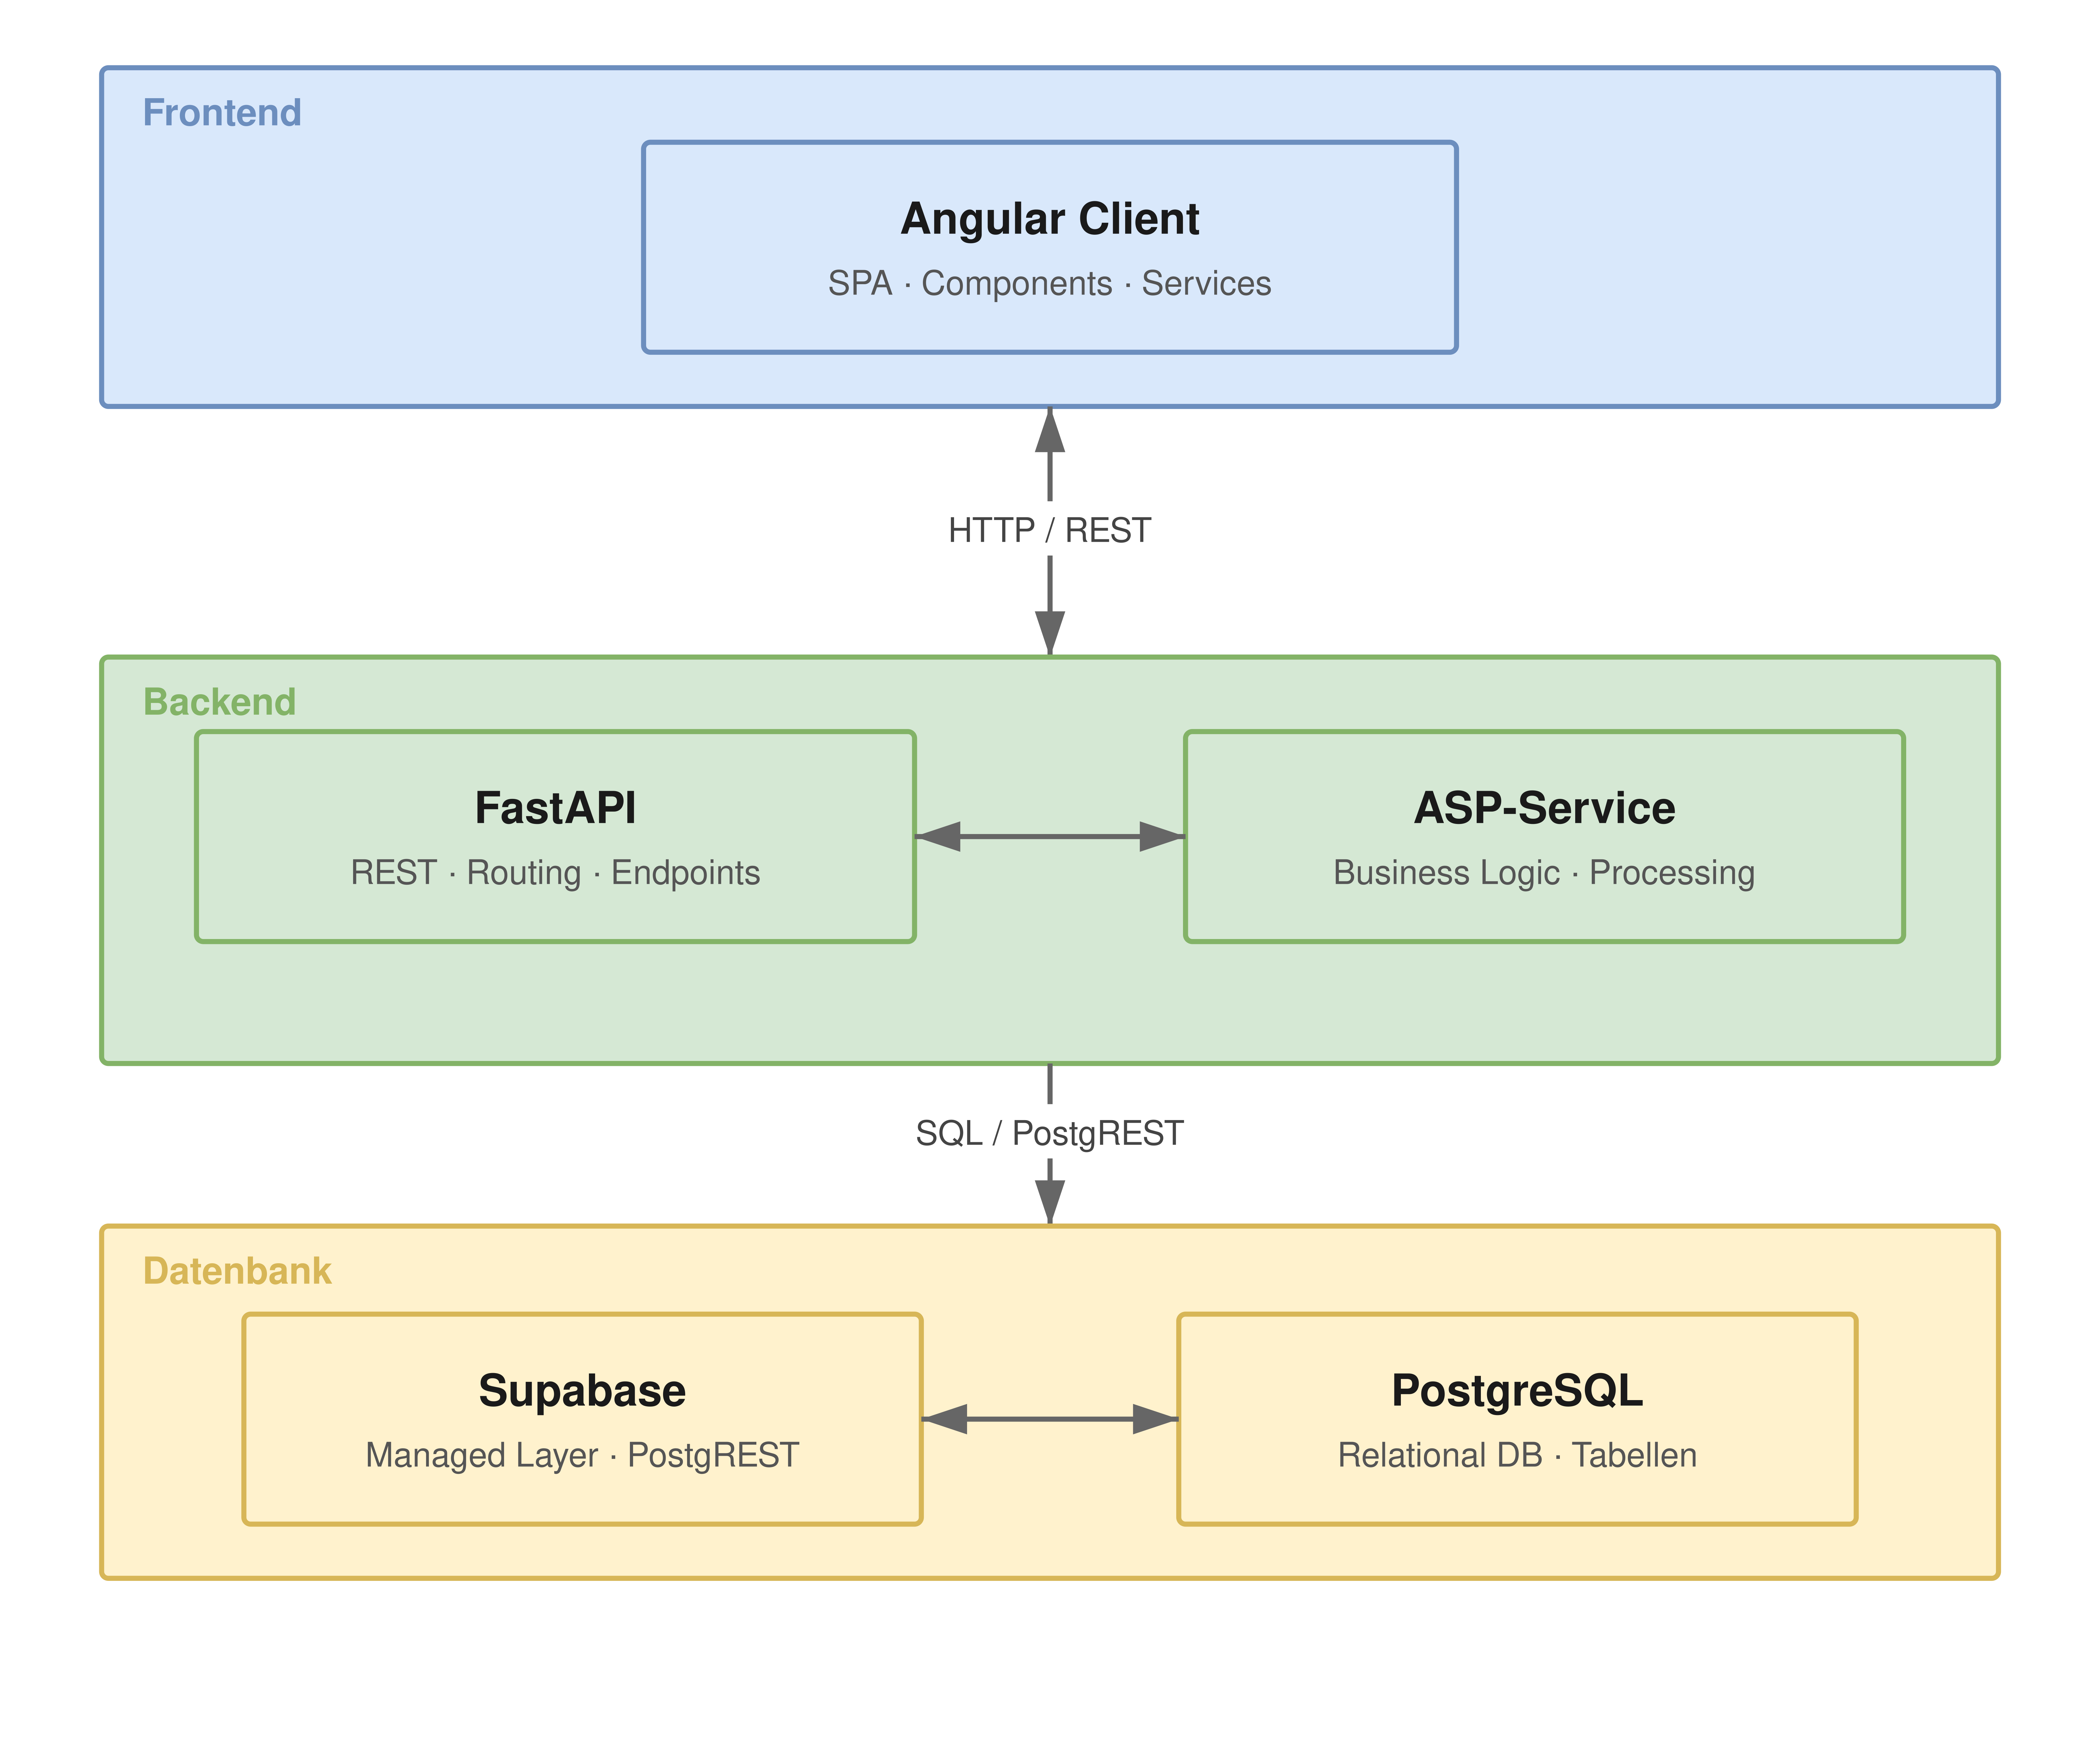
\includegraphics[width=\linewidth]{images/architecture}
	\caption{
		Applikations-Architektur
	}\label{fig:Applikations-Architektur}
\end{figure}

Das Frontend wurde als Single-Page Application mit dem Angular Framework umgesetzt. Es stellt die Benutzeroberfläche bereit, über die Mitarbeiter, Stationen, Kompetenzen verwaltet, sowie Constraints festgelegt und Monatspläne angezeigt werden können. Die Kommunikation mit dem Backend erfolgt ausschließlich über HTTP-REST-Schnittstellen.
Das Backend ist in Python mit FastAPI realisiert und übernimmt die gesamte Geschäftslogik der Anwendung. Es stellt REST-Endpunkte bereit und verarbeitet eingehende Anfragen Ein zentraler Bestandteil des Backends ist der ASP-Service. Dieser Service ist für die Berechnung der Monatspläne unter Berücksichtigung der definierten Hard und Soft Constraints verantwortlich.
Als Datenbankschicht wird Supabase eingesetzt, eine Open-Source-Plattform, die auf PostgreSQL aufbaut. Supabase stellt neben der relationalen Datenbank auch eine PostgREST-Schnittstelle bereit, über die das Backend direkt auf die Datenbankressourcen zugreifen kann.

\section{Datenmodell}
\subsection{Entitäten}
In \autoref{fig:Datenmodell} wird das Datenmodell dargestellt. Im Folgenden wird auf die Struktur der Daten eingegangen. 

\texttt{users} repräsentiert die Mitarbeitenden des Systems. Neben einem Primärschlüssel (\texttt{id}) wird auch der Name (\texttt{name}) persistiert. Die Entität dient als Ankerpunkt für Qualifikations- und Zuweisungsbeziehungen.

\texttt{skills} bildet die Menge verfügbarer Kompetenzen ab. Jede Kompetenz beinhlatet eine \texttt{id} und einen \texttt{name}.

\texttt{stations} modelliert die Arbeitsstationen, denen Benutzer zugewiesen werden können. Das Attribut \texttt{maxAssignments} legt die maximale Anzahl gleichzeitiger Zuweisungen pro Station fest und stellt damit eine wichtige Kapazitätsbeschränkung dar.

Durch die Tabelle \texttt{schedules} ist es möglich, \texttt{Assignments} zu Diensplänen zuzuweisen und diese und anhand der Attribute \texttt{year} und \texttt{month}  zeitlich einzuordnen. Mit dem Boolean \texttt{is\_loaded}  wird gespeichert, welcher Dienstplan aktuell im Kalender geladen ist.

\subsection{Assoziationstabellen}
\texttt{user\_skills} bildet die m:n-Beziehung zwischen \texttt{users} und \texttt{skills} ab. Dadurch kann gespeichert werden, über welche Qualifikationen ein Benutzer verfügt. Die Tabelle besteht ausschließlich aus den beiden Fremdschlüsseln \texttt{user\_id} und \texttt{skill\_id}.

Die Tabelle \texttt{station\_skills} definiert, welche Fähigkeiten für eine bestimmte Station erforderlich sind, und bildet somit eine m:n-Beziehung zwischen \texttt{stations} und \texttt{skills}. Eine Station kann dabei mehrere benötigte Qualifikationen besitzen. Dadurch wird ein Abgleich zwischen den Fähigkeiten der Benutzer und den Anforderungen der Stationen ermöglicht.

\texttt{station\_assignments} stellt die zentrale Tabelle des Datenmodells dar. Sie verbindet eine Station (\texttt{station\_id}) mit einem Benutzer (\texttt{user\_id}) sowie einem Dienstplan (\texttt{schedule\_id}) für ein bestimmtes Datum (\texttt{date}). Das Attribut \texttt{user\_id} ist optional, wodurch auch Platzhalter-Zuweisungen abgespeichert werden können, falls ein Dienstplan nicht für jede Station einen Mitarbeiter zuweisen kann.

\begin{figure}[h]
	\centering
	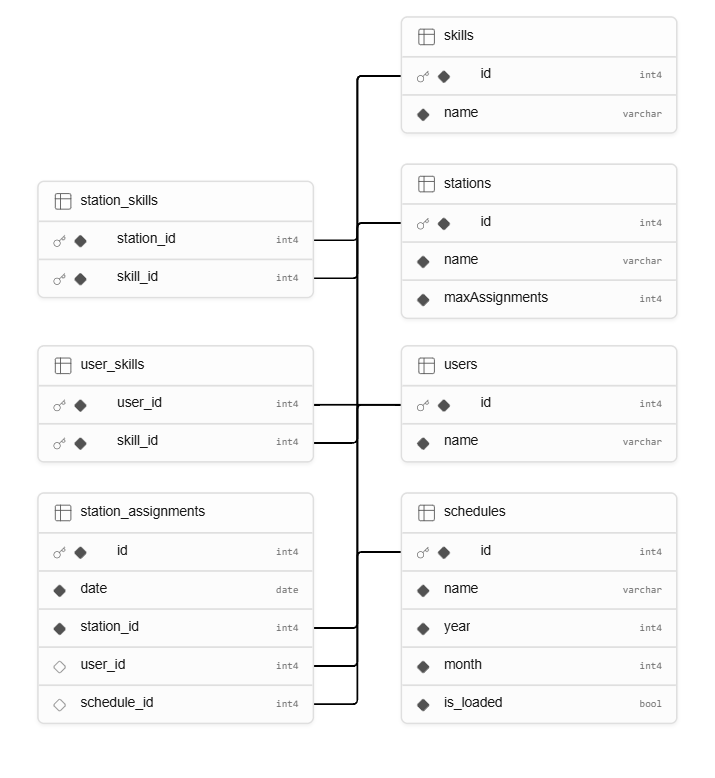
\includegraphics[width=\linewidth]{images/datenmodell}
	\caption{
		Datenmodell
	}\label{fig:Datenmodell}
\end{figure}

%% 
%%%%%%%%%%%%%%%%%%%%%%%%%%%%%%%%%%%%%%%%%%%%%%%%%%%%%%%%%%%%%%%%%%%%%%%%%%%%%%%%
